\documentclass{memoir}
\usepackage{hyperref}
\usepackage{graphicx}
\graphicspath{ {figures/} }

\setcounter{secnumdepth}{3}

\title{Distributed Systems:\\Crossing Intersection with Autonomous Vehicles}

\author{Antonio Toncetti\\Gabriele Venturato\\\\DMIF, University of Udine, Italy}

\date{%Version 0.1, 
	\today}

\begin{document}


%\begin{titlingpage}
\maketitle
\begin{abstract}
The aim of this project is to provide an implemented solution to the problem of autonomous vehicles crossing an intersection.
Although the solution relies on some simplifications, it can be further elaborated to work in a real-case scenario.

The solution proposed in this report is meant to be more general and as modular as possible, in order for it to be possibly extended in a concrete situation.
\end{abstract}
%\end{titlingpage}

\chapter{Introduction}\label{ch:intro}

The problem to solve is the one in which some autonomous vehicles have to cross an intersection without getting involved in road accidents. 

The idea is to solve the problem for a generic intersection. The autonomous vehicles can not rely on a central server, they have to cooperate with each other to cross the intersection by taking decisions which ensure a \emph{fair} and \emph{safe} policy. In particular there are two components in the proposed solution: vehicles and the environment. The latter is necessary in this context in order to simulate sensors that are usually inside autonomous vehicles which allows them to interact with the environment (e.g. proximity sensors, GPS, cameras, etc\dots).
The system is \emph{fault tolerant}, but neither byzantine processes nor cybersecurity hazards are taken in consideration, for simplification purposes.

The report starts by analysing the project: Chapter~\ref{ch:analysis} is devoted to use cases, functional and non-functional requirements, and system assumptions too. Chapter~\ref{ch:project} contains the description of the general architecture, and specific algorithms.

Following chapters aim to describe details of the implementation, and validation w.r.t. requirements.



\chapter{Analysis}\label{ch:analysis}

This chapter describes in detail some fundamental assumptions about the system, as well as functional and non-functional requirements.

\section{Use cases}

\subsection{Vehicle at an intersection}
\begin{description}
	\addtolength{\itemindent}{0.5cm}
	\item[Brief Description] \hfill \\
	An Autonomous Vehicle (AV) is approaching, entering and leaving a non empty intersection. The use case begins with the AV approaching an intersection and ends with the AV having left the intersection in the desired direction. 
	
	\item[Actors] \hfill
	\begin{itemize}
		\item Autonomous Vehicles (AVs)
		\item Environment
	\end{itemize}
	
	\item[Preconditions] \hfill
	\begin{itemize}
		\item There is more than one AV at the intersection. 
		\item AVs can be both active and inactive.
		\item The AV approaching the intersection is active.
		\item The AV knows the direction (exit) to take.
	\end{itemize}
	
	\item[Scenarios] \hfill
	\begin{description}
		\item Main scenario
		\begin{enumerate}
			\item The AV is travelling along a road leading to an intersection.
			\item The AV is approaching the intersection.
			\item The AV stops at the entrance to the intersection.
			\item The AV signals its intent to other AVs at the intersection.
			\item The AV agrees with the other participants on how to solve the intersection.
			\item The AV initiates the turn procedure towards the desired exit.
			\item The AV is in the intersection travelling to an exit.
			\item The AV leaves the intersection through an exit.
			\item The AV signals that it has successfully left the intersection.
			\item The AV continues to travel along its path.
		\end{enumerate}
		\item Alternative scenario
		\begin{enumerate}
			\item 1, 2	The AV finds an active AV in front and gets in the queue.
			\item 1, 2	The AV finds a faulty AV in front and overtakes him.
			\item 6. 7	The AV finds a faulty AV and awaits for its removal.
		\end{enumerate}
	\end{description}

	\item[Postconditions] \hfill \\
	At any point in its journey the AV can become inactive due to a mechanical failure or  a software failure.
\end{description}

\subsection{Vehicle mechanical failure}
\begin{description}
	\addtolength{\itemindent}{0.5cm}
	\item[Brief Description] \hfill \\
	When an Autonomous Vehicle (AV) has a mechanical failure but the software is still working properly. The use case begins when the failure happens, and ends with the recovery of a normal situation.
	
	\item[Actors] \hfill
	\begin{itemize}
		\item Autonomous Vehicle (AV)
		\item Environment
	\end{itemize}
	
	\item[Preconditions] \hfill
	\begin{itemize}
		\item There is at least one AV with a mechanical fault.
		\item There are possibly other AVs in the intercept network.
		\item Any other AV can fail at any moment.
	\end{itemize}
	
	\item[Scenarios] \hfill
	\begin{description}
		\item Main scenario
		\begin{enumerate}
			\item The AV detects the mechanical fault.
			\item The faulty AV communicates its state to the others in the network and to the environment.
			\item Faulty AV awaits until it is removed.
			\item Before leaving, communicate to the others (and the environment) the resolution.
		\end{enumerate}
	\end{description}
	
	\item[Postconditions] \hfill \\
	The network does not contain the faulty AV anymore.
\end{description}

\subsection{Vehicle software failure}
\begin{description}
	\addtolength{\itemindent}{0.5cm}
	\item[Brief Description] \hfill \\
	When an Autonomous Vehicle (AV) has a software failure. This implies a mechanical failure, because we assume that a software failure stops the AV. The use case begins with the fault having happened, and ends with the recovery of a normal situation.
	
	\item[Actors] \hfill
	\begin{itemize}
		\item Autonomous Vehicle (AV)
		\item Environment
	\end{itemize}
	
	\item[Preconditions] \hfill
	\begin{itemize}
		\item There is at least one AV with a software fault.
		\item There are possibly other AVs in the intersection network.
		\item Any other AV can fail at any moment.
	\end{itemize}
	
	\item[Scenarios] \hfill
	\begin{description}
		\item Main scenario
		\begin{enumerate}
			\item One of the other AVs in the network detects the fault.
			\item The AV which detects the fault communicates to others in the network which AV has just faulted.
			\item Everyone awaits for the faulty AV to be removed.
			\item The Environment communicates to the AVs in the network the occured removal.
		\end{enumerate}
		\item Alternative scenario
		\begin{enumerate}
			\item On 1 can happen that there is no other AVs, in that case the faulted AV stays into the intersection until someone comes to the rescue.
		\end{enumerate}
	\end{description}
	
	\item[Postconditions] \hfill \\
	The network does not contain the faulty AV anymore.
\end{description}

\section{Assumptions}

Some general considerations are here presented. First of all it is assumed a situation in which each autonomous vehicle knows its destination and the roads it is going to travel, since we can assume that each autonomous vehicle has a GPS device on board.

Moreover it is assumed, for sake of simplicity, that all vehicles have the same dimension --- or better: that each vehicle can fit into a single position of the internal model used to represent the roads. Moreover, common physical quantities (like weight, speed, acceleration, etc\dots) are omitted. Instead, the autonomous vehicles move in unit steps governed by the internal model.
\newline

Further assumptions are:

\begin{itemize}
	\item \emph{Faults}: at any moment a failure can arise in vehicles --- software or mechanical. A mechanical failure does not compromise the software abilities, but a software failure implies a mechanical failure. So we can assume that if the software fails, the autonomous vehicle stops and goes in ``emergency mode''. It is also assumed that if a crash happens, it must be managed by removing the faulty vehicle with a tow truck (or something similar).
	\item \emph{Moves}: the path that a vehicle can take inside the interception is predefined and known a priori. From each position there is a unique path to each destination, and no one can modify or choose a different path once decided. A visual representation of this assumption can be found in Figure~\ref{fig:intersection-graph}, in which green dots represent positions occupied while crossing, and light-blue dots are the destinations. Once a vehicle reaches its destination, it is considered ``satisfied'', and can not fail anymore, it can only move forward on its own way. Reversing is not allowed.
	\item \emph{Message Delivery}: each vehicle can communicate with its immediate neighbors, i.e. the vehicle in front, the one behind it, and if it is at the verge of the crossroads, it can communicate with the others at the verge, and with crossing vehicles. Therefore it's assumed that there exist an upper bound time in message passing between two vehicles. This is justified by the fact that all connection are almost direct, without routers or broker that can cause bottle-necks or network congestion.
\end{itemize}

\begin{figure}
	\centering
	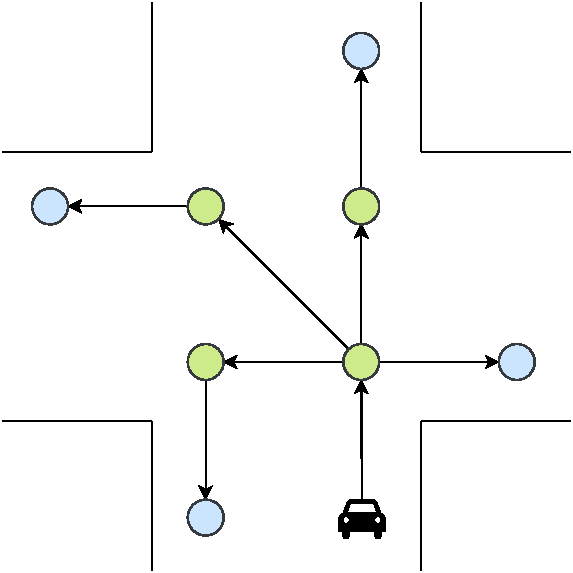
\includegraphics[width=0.4\linewidth]{intersection_graph.pdf}
	\caption{Example of predefined movements that a vehicle can follow in crossing an intersection.}
	\label{fig:intersection-graph}
\end{figure}

\section{Functional requirements}
The solution provides two main modules: \emph{vehicle} and \emph{environment}. Also a \emph{vehicle generator} is provided, in order to test and validate the solution proposed.

\subsection{Vehicle}
Each vehicle has an internal state at any moment. Moreover it:

\begin{itemize}
	\item knows its position and what happens around, through the environment (in a real context this is handled by sensors like GPS and proximity sensors): it can detect if there are other vehicles trying to cross, or if there is a vehicle in front or behind it.
	\item communicates with its neighbors by sharing: the direction it wants to travel, its internal state, the next position he is about to reach.
	\item if it is in the queue, it knows nothing else than its internal information and that it is taking part in a queue with someone before and possibly behind. It can communicate only with these two.
	\item if it is at the head of the queue, it can connect with other vehicles (that are at the head of other queues) that are crossing the intersection.
\end{itemize}
Therefore the main functions offered by this module are:

\begin{itemize}
	\item \texttt{startup()} to start the vehicle.
	\item \texttt{stop()} to stop the vehicle.
	\item \texttt{cause\_mechanical\_failure()} and \texttt{cause\_software\_failure()}, to cause failures; these are useful in testing to simulate failures.
	\item \texttt{send\_message(To,Msg)} to communicate with other vehicles.
	\item \texttt{move()} to move one step forward.
	\item \texttt{check\_next\_position()} to check if the position it is willing to move is free.
\end{itemize}


\subsection{Environment}
The environment represent the vehicle ability to use its sensors. It knows the intersection shape and dimension; it knows vehicles approaching the crossroads and the ones in the queues; it provides vehicles with all the information they need to safely circulate within the environment.

The main functions offered by this module are:

\begin{itemize}
	\item \texttt{is\_position\_free(Pos)} to simulate proximity sensors; check if a specific position is free.
	\item \texttt{update\_position(Vehicle,OldPos,NewPos)} to update its internal state moving the vehicle from the old position into the new one.
	\item \texttt{get\_route(StartPos,DestPos)} to simulate the GPS; a vehicle that is starting its journey asks the environment which is the route it has to travel.
	\item \texttt{get\_participants()} to simulate proximity sensors, cameras, and antennas; to ask the identity of vehicles at the verge of the intersection. 
\end{itemize}

\section{Non functional requirements}
The system does not handle byzantine processes nor cybersecurity issues.

\begin{itemize}
	\item \emph{Safeness}: there can not be more than a vehicle in the same position at the same time;
	\item \emph{Liveness}: if a vehicle approaches the intersection and is waiting to cross it, it will eventually cross it;
	\item \emph{Fairness}: if a vehicle approaches the intersection and is waiting to cross it, there exists a bound to the waiting time;
	\item \emph{Fault Tolerant}: the system is tolerant to mechanical and software failures;
	\item \emph{Distributed}: there is no central server, vehicles have to coordinate each other.
\end{itemize}



\chapter{Project}\label{ch:project}
This chapter is devoted to the description of the general architecture, and specific algorithms.

\section{Logical architecture}
The solution relies on two main modules, and a secondary one for tests.

\begin{itemize}
	\item \emph{Vehicle}: represented as a finite state automaton. A graphical representation can be seen in Figure~\ref{fig:vehicle-automaton}. Each state represents a situation in which the vehicle can find itself. A vehicle is in the \emph{Init} state when it has just approached the intersection. It is in the \emph{Ready} state when it is at the verge and has identified the participants. It is in \emph{Election} when it is performing the election algorithm to choose who will be the one to cross. \emph{Crossing} when it is crossing the interception, and \emph{Terminate} when it has finished the crossing. When a mechanical failure happens, it notifies the event to its neighbors and then terminate; so a crash state is not needed.
	\item \emph{Environment}: represents the physical environment accessible through the autonomous vehicle's sensors.
	\item \emph{Vehicle Generator}: a module aimed to (pseudo-)randomly generate vehicles that approach the intersection, and it is used to test and validate the proposed solution.
\end{itemize}

\begin{figure}
	\centering
	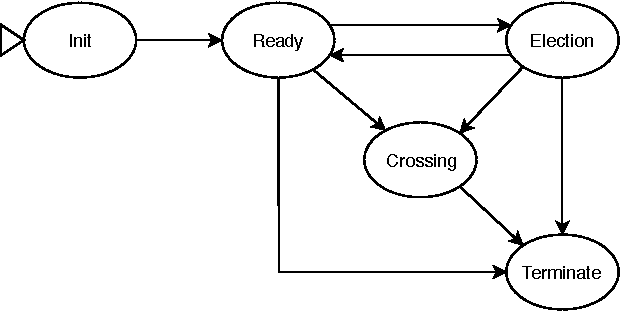
\includegraphics[width=0.8\linewidth]{vehicle_automaton.pdf}
	\caption{Vehicle as a finite state automaton.}
	\label{fig:vehicle-automaton}
\end{figure}

\section{Protocols and algorithms}
This section describes the algorithm to solve the core part of the project. Moreover, some peculiar situation sequence diagrams are presented.

\subsection{Intersection Crossing Algorithm}
Vehicles queue up along the roads leading to an intersection awaiting for their turn to cross. The first vehicle of a queue is the vehicle at the verge of entering the intersection and we will call such vehicle a \emph{participant} of the intersection crossing algorithm.

Note that this algorithm applies to generic intersections, just by adapting the representing graph. Moreover, it trivially guarantees the \emph{fairness} and \emph{liveness} requirements (thus it is also \emph{deadlock-free}), thanks to its round robin characteristic.
\\\\
\noindent
The algorithm maintains the following invariant through execution:

\begin{itemize}
	\item one working (i.e. without faults) vehicle per time can be crossing the intersection
	\item only the leader vehicle can cross the intersection
\end{itemize}
Algorithm description:
\begin{enumerate}
	\item The participants (first vehicles in their respective queues) are willing to cross the intersection;
	\item They start a slightly modified version \footnote{In the canonical version of the Bully Algorithm, every participant is supposed to know other IDs a priori. The version used here does not rely on this assumption. Still, it guarantees the same outcome, even w.r.t. non functional requirements (safety and liveness).} of the Bully Algorithm to elect a leader: it terminates with the leader $L$, and the next leader $L'$, which is the first vehicle after him in a clockwise manner;
	\item $L$ begins to cross the intersection;
	\item After $L$ has successfully crossed the intersection, the participants are informed;
	\item $L'$ identifies the next leader $L''$ by choosing the first vehicle after him in a clockwise manner;
	\item The lead passes to $L'$ informing every participant that it's the new leader;
	\item The algorithm repeats from 3, where $L = L'$ and $L' = L''$.
\end{enumerate}
Additional details:
\begin{itemize}
	\item After the leader election, every participant knows who is the current leader, but only the leader knows who is the next one. In this way if the leader dies, it is necessary to perform a new election;
	\item Once the leader starts crossing, the vehicle behind it (if any) becomes a new participant and asks to join the algorithm. Only the leader answers, providing its identity.
	\item If a vehicle approaches an empty intersection it automatically elect itself as leader and starts the crossing.
\end{itemize}
A leader election starts only when new participants do not receive an answer when asking to join the algorithm; or when, after the leader is gone (after completing the crossing, or due to a failure), remaining participants does not receive the message from the candidate, communicating it is the new leader.

\subsubsection{Managing abnormal cases}

All participants monitor only the leader, if it fails, everyone is expecting a message from the candidate, telling it is the new leader. If this not happens, a new election is started. Moreover:

\begin{itemize}
	\item If the leader fails, the vehicle in clockwise order after him becomes the new leader --- identifying also the next candidate leader --- and the algorithm restarts from 3.
	\item If the leader fails while crossing, a timeout $T$ is needed before it is removed from the intersection. Meanwhile a new election can start, and the new leader can start crossing, but it has to stop if the position in front of him is still occupied from the previous faulty leader, until the position gets liberated.
	\item Some peculiar situations can happen for example when a new vehicle arrives at the interseption while the leader is gone and it is passing the lead to the candidate. It the new vehicle arrives at this unfortunate moment, it could receive no answers when asking who is the leader, and so it starts a new election. The risk is that the candidate can become leader, and after a while someone else can win the election, stealing its role of leader. This can lead to disastrous scenarios, in which more than a vehicle starts crossing. To avoid this, it is \emph{necessary} that a candidate receiving the role from the previous leader, in case of a sudden election, it turns out to be the winner. So, no one can steal the lead from anyone else. This is guaranteed with an appropriate implementation, described in the next chapter.
\end{itemize}

\subsection{Sequence Diagrams}
This section presents some sequence diagrams of relevant case situations.

\subsubsection{Normal execution of Intersection Crossing Algorithm}
The diagram in Figure~\ref{fig:seq-diag-crossing-intersection} represent the normal execution of the algorithm described above. It starts at the end of the Bully Algorithm, with the $AV_4$ communicating it is the leader. It is assumed the queues are enumerated from 1 to 4 in clockwise order.

The leader crosses the intersection by asking the environment if the position in front of it is free, and continues to cross until it reaches its destination.

It is important to note that when the leader starts crossing, $AV_5$ --- which is the one following $AV_4$ in the queue --- moves forward. Then $AV_5$ is at the verge of the intersection and can communicate with the other participants in order to compete for the crossing.

\begin{figure}
	\centering
	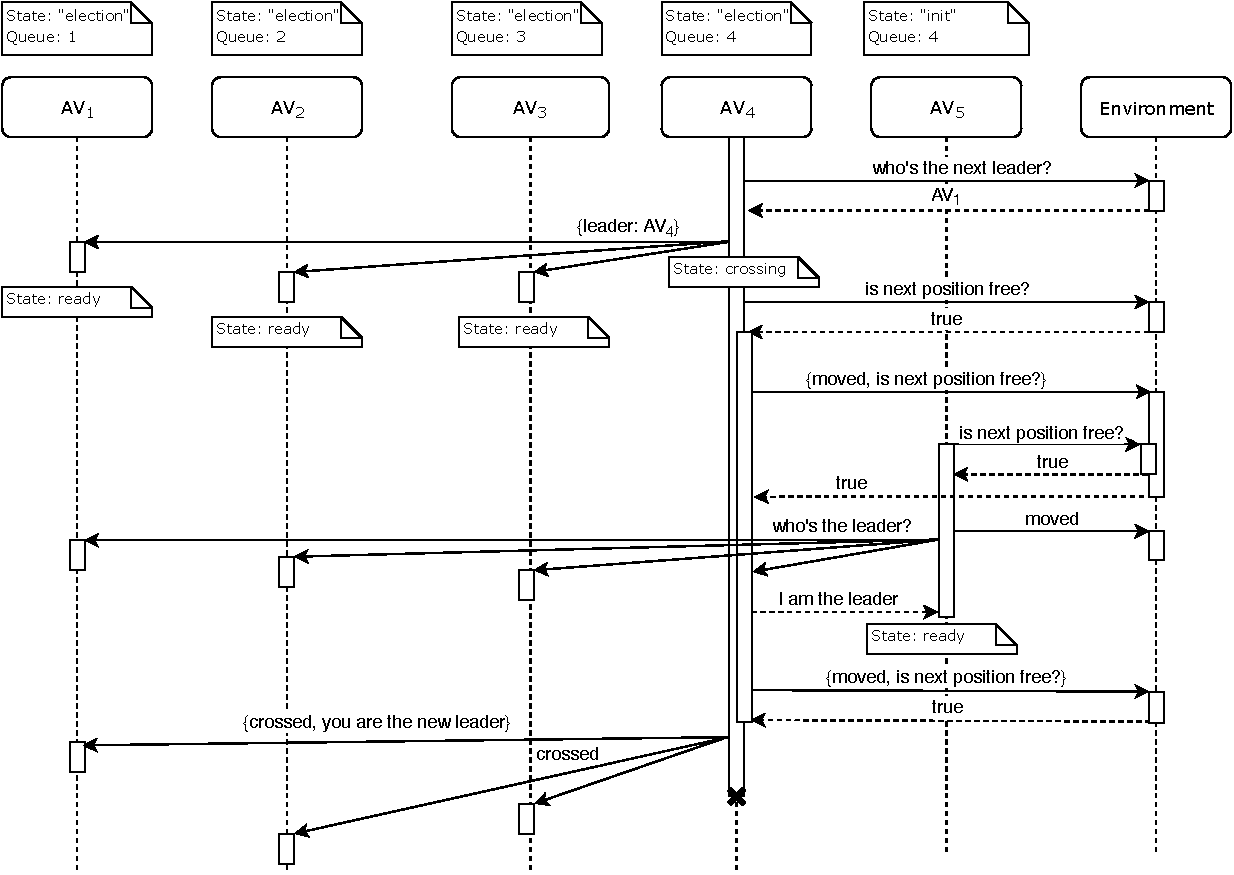
\includegraphics[width=\linewidth]{sequence_diagrams/crossing_intersection.pdf}
	\caption{Sequence diagram on a normal execution of the Intersection Crossing Algorithm described above.}
	\label{fig:seq-diag-crossing-intersection}
\end{figure}

\subsection{Dealing with AV failures}

When the leader dies because of a software failure, it can not promote the candidate. So a new election is needed. The situation is represented by the sequence diagram in Figure~\ref{fig:seq-diag-leader-sw-failure}

\begin{figure}
	\centering
	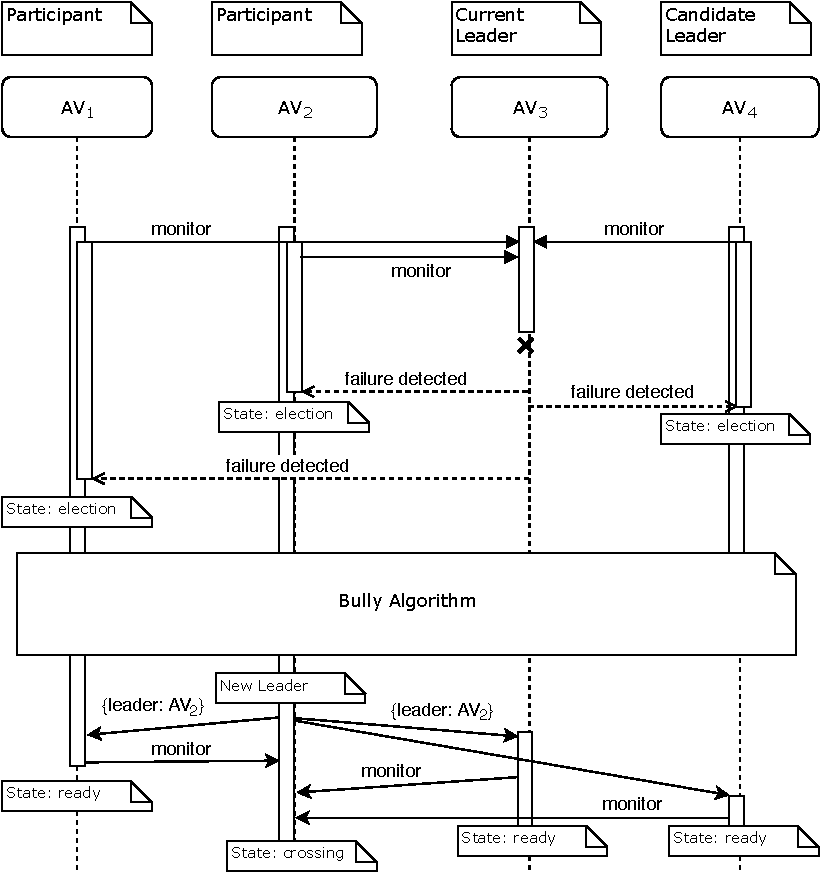
\includegraphics[width=\linewidth]{sequence_diagrams/leader_sw_failure.pdf}
	\caption{Sequence diagram representing a generic leader failure.}
	\label{fig:seq-diag-leader-sw-failure}
\end{figure}

The last situation in Figure~\ref{fig:seq-diag-candidate-failure} represents a failure of the candidate leader. When the leader finish the crossing, everyone wait a timeout $T$ for a message from the candidate. Since it is not alive, the timeout runs out, and a new election is performed.

\begin{figure}
	\centering
	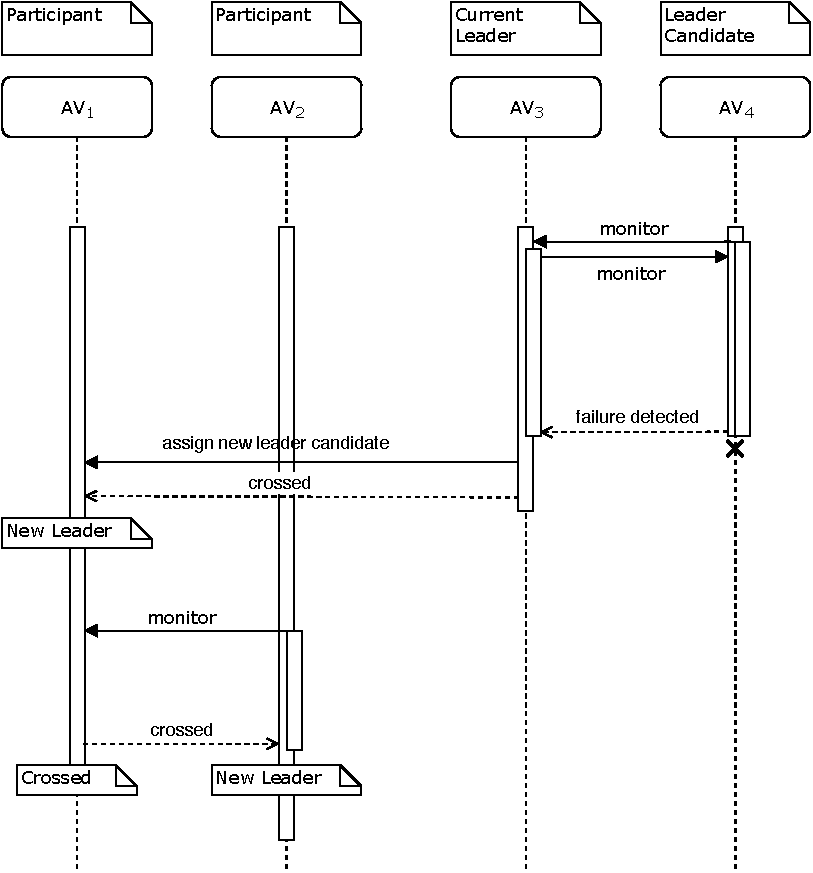
\includegraphics[width=\linewidth]{sequence_diagrams/candidate_failure.pdf}
	\caption{Sequence diagram of a candidate leader failure.}
	\label{fig:seq-diag-candidate-failure}
\end{figure}

\section{Physical architecture and deployment}
The architecture is quite simple, a graphical representation is displayed in Figure~\ref{fig:physical-architecture}. Each Autonomous Vehicle (AV) is a physical node. The Environment represents the world sensed by AVs, so it is on a separate node, together with the vehicle generator. AVs can ask the environment for information, and they can communicate with their neighbors \footnote{For a definition of ``neighbors'', see in Chapter~\ref{ch:analysis}, in assumptions section. Where the message delivery assumption is described .}.

\begin{figure}
	\centering
	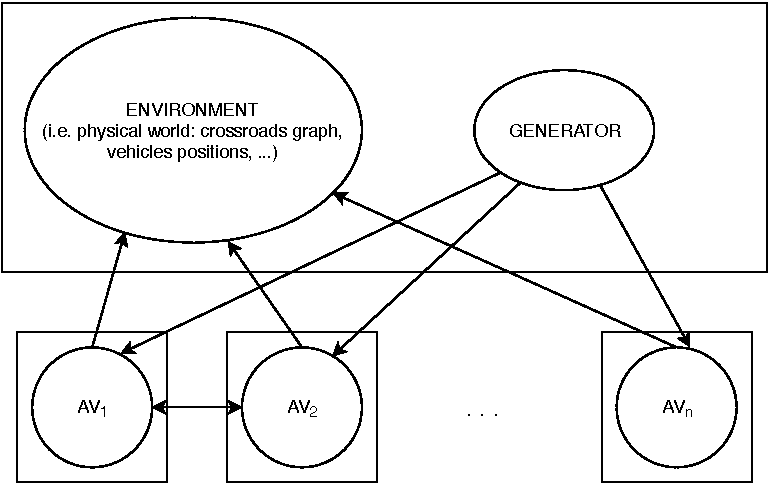
\includegraphics[width=0.8\linewidth]{physical_architecture.pdf}
	\caption{Physical architecture: Environment, Generator, and Autonomous Vehicles (AV).}
	\label{fig:physical-architecture}
\end{figure}


\chapter{Implementation}
The project is developed in \href{https://www.erlang.org/}{Erlang}.

\begin{figure}
	\centering
	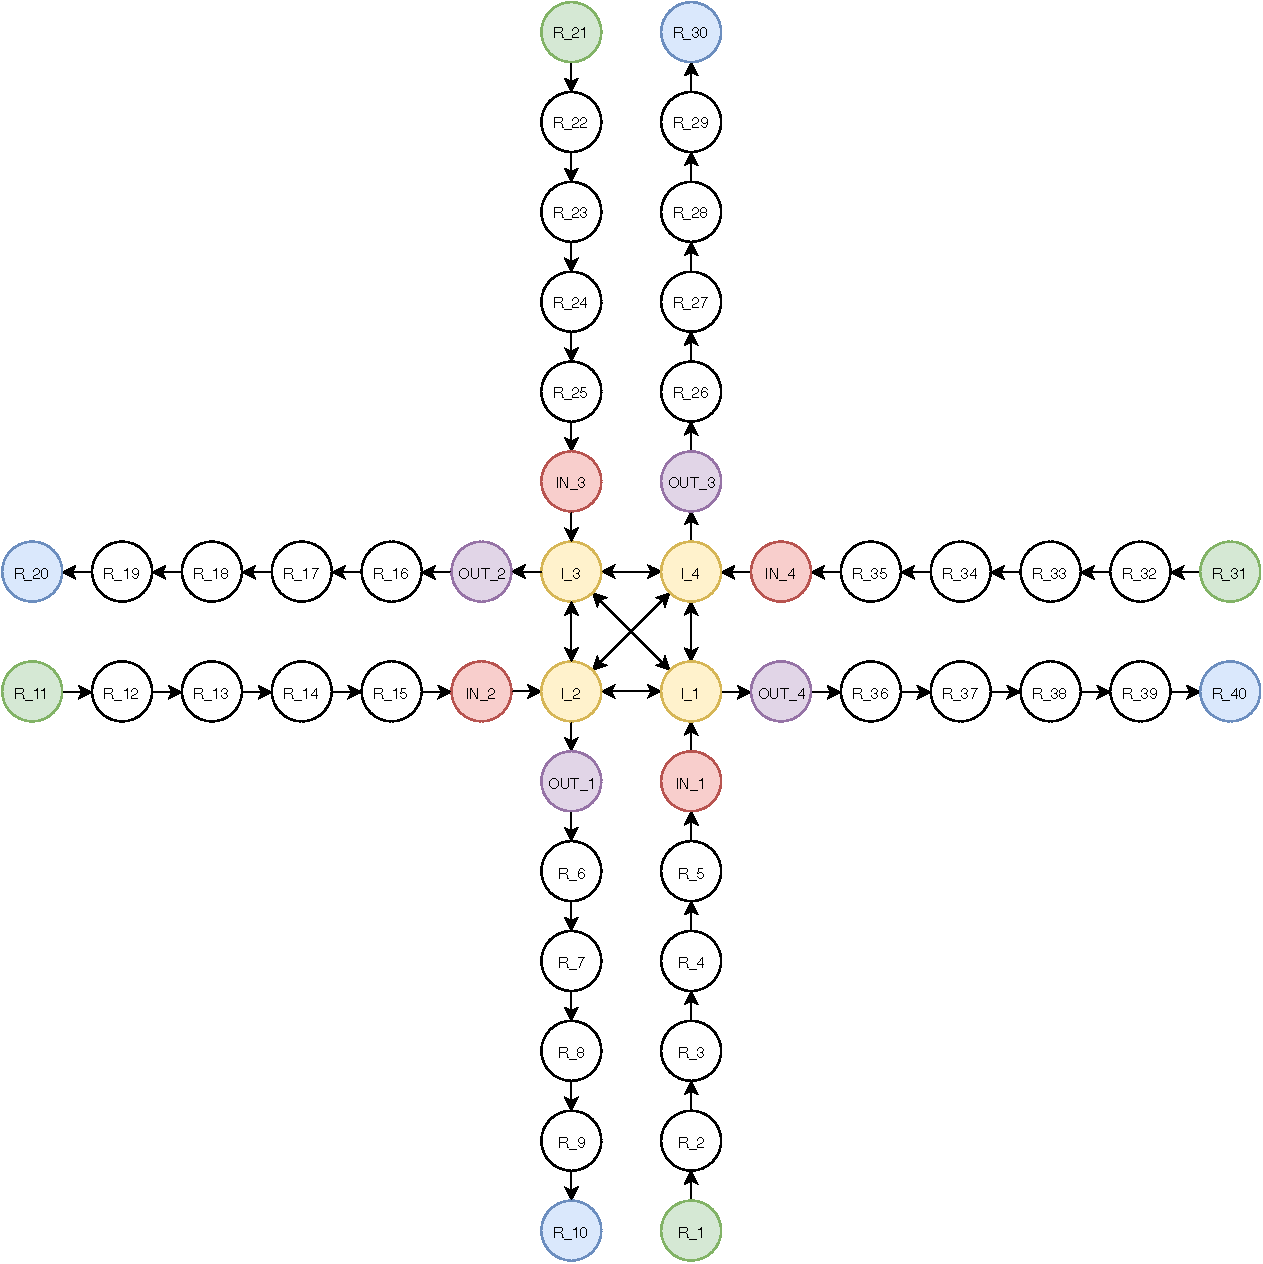
\includegraphics[width=\linewidth]{config_graph.pdf}
	\caption{Graphical representation of the intersection graph contained in the configuration file, and used to test the project. Nodes with name $R\_x$ represents roads. Details: in green start nodes ($R\_1, R\_11, R\_21, R\_31$), in blue destination node ($R\_10, R\_20, R\_30, R\_40$), in yellow intersection internal nodes ($I\_x$), in red intersection entrance nodes ($IN\_x$), in purple intersection exit nodes ($OUT\_x$). }
	\label{fig:config-graph}
\end{figure}

\section{Getting Started}
\subsection{Project Structure}
\subsection{Hands On}

\section{Development Details}

\subsection{Vehicle system}

The vehicle system architecture follows the event-based multi-agent architecture where the only source of events are vehicles (agents) and the environment.
Such architecture will greatly help in dealing with accidental complexity, changing requirements, security and performance.


Vehicles represent the main source of events, autonomously driving control towards their own goals, and producing internal events through their actions.
The environment and other vehicles model the external events. External events are captured by the vehicle's devices such as sensors, sonars, camera systems, receivers, transmitters, etc.

\begin{figure}
	\centering
	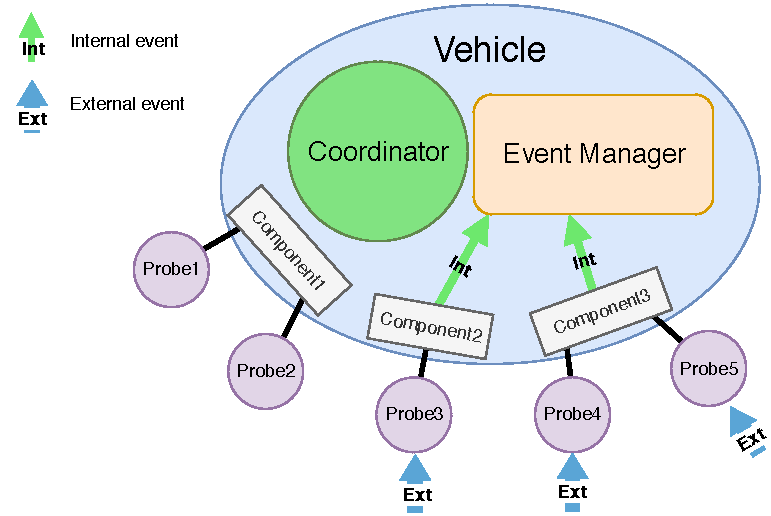
\includegraphics[width=0.7\linewidth]{implementation_details/vehicle_high-level_architecture.pdf}
	\caption{Vehicle system architecture: Coordinator, Event Manager, and Components with Probes attached.}
	\label{fig:vehicle-architecture}
\end{figure}

The main elements of the architecture are the Coordinator, the Event Manager and various components that provide a specific service.
Vehicle components communicate by producing and receiving event notifications. All of the vehicle's functionality is split among the components: each component is responsible for delivering a specific service to the vehicle.

Components can be connected to sensors and other external devices in order to successfully deliver their functionality. External devices are referred to as probes.
The responsibility of probes is to collect external events from the environment or other vehicles and forward them to the component to which they are attached to.
External events received by components and translated them into internal events.


The Coordinator listens to specific internal events in order to coordinate the components to reach the vehicle's goal.

\subsection{Architecture elements}

This subsection presents the architectural elements: Event Manager, Components and the Coordinator. Figure ~\ref{fig:erlang-point-of-view} shows the supervision tree implemented in Erlang with all the architectural elements.

\begin{figure}
	\centering
	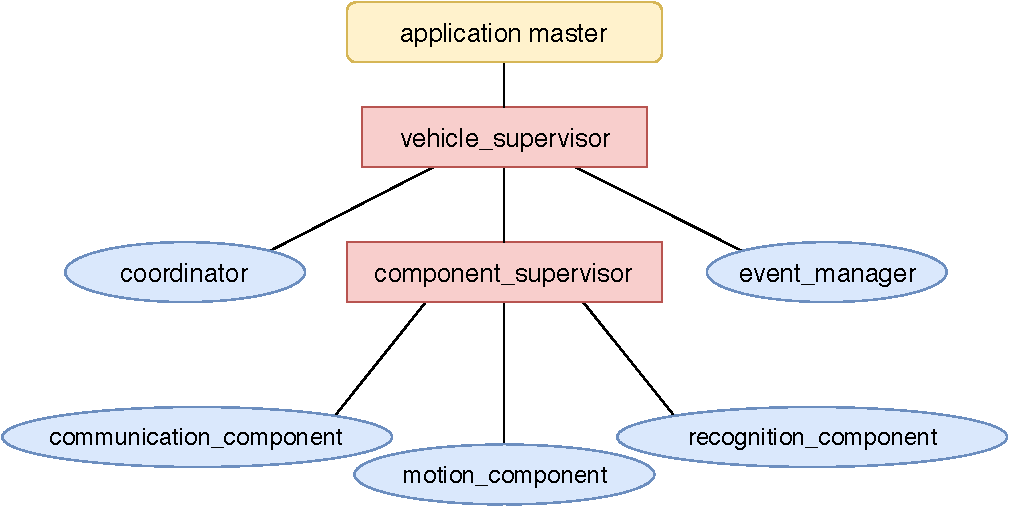
\includegraphics[width=0.8\linewidth]{implementation_details/erlang_point-of-view.pdf}
	\caption{The implemented vehicle system supervision tree (Erlang point of view).}
	\label{fig:erlang-point-of-view}
\end{figure}

\subsubsection{Event Manager}

Components communicate by sending event notifications to the Event Manager.
Being not real messages, events have not a designed receiver: they are distributed by the Event Manager to Components that subscribed to that sort of events.

The Event Manager acts as a middleware, inverting the logic of program execution, where a component does not need to know the existence of other components to provide its service and thus facilitatates the addition of new features and components.

\subsubsection{Components}

Components are the only providers of functionality. Each component delivers a specific functionality to the system.

Components can be \textit{passive} or \textit{active}. Passive components do not generate internal events and their sole purpose is to listen to internal events and act accordingly. An example of a passive component is the Logging Component which listens for specific internal events and logs them onto a file.

Active components are components that generate internal events. For example the Communication Component, whose sole purpose is to handle communication between vehicles, is required by components that need Vehicle-to-Vehicle (V2V) communication services.
\\

\textit{Note that both active and passive components are capable of performing actions, changing their state and communicating with their devices except that passive components cannot interfere with the event flow of the vehicle because they don't generate internal events.}
\\

Components can have multiple devices attached (sensors, receivers, transmitters, etc.) in order to detect external events and provide their functionality.

Components help to address the issues of event aggregation and transformation by making event notifications meaningful at the level of interpretation required for making other components activities effective. They effectively act as event mediators (or, correlators), translating external events into meaningful internal events.
\\
\newline
\textbf{Component Structure}
\\
\newline
The structure of a component consists of: 
\begin{itemize}
	\item component module (mandatory)
	\item event listener (optional)
\end{itemize}

\underline{The component module:}
\\
The component module maintains all the logic related to the specific service it is built for, for example a component in charge of the navigation system deals with navigation related tasks only.

The component module can be connected to zero or more devices in order to provide its services, for example the navigation component can use a GPS device to gather geolocation data. 
\\

When needed, components can spawn additional processes called Actions to perform more advanced and complicated tasks (Actions can also be used for enabling the selection of algorithms at runtime, effectively letting the algorithm vary independently from the component, a strategy pattern in OO terms).

\begin{figure}
	\centering
	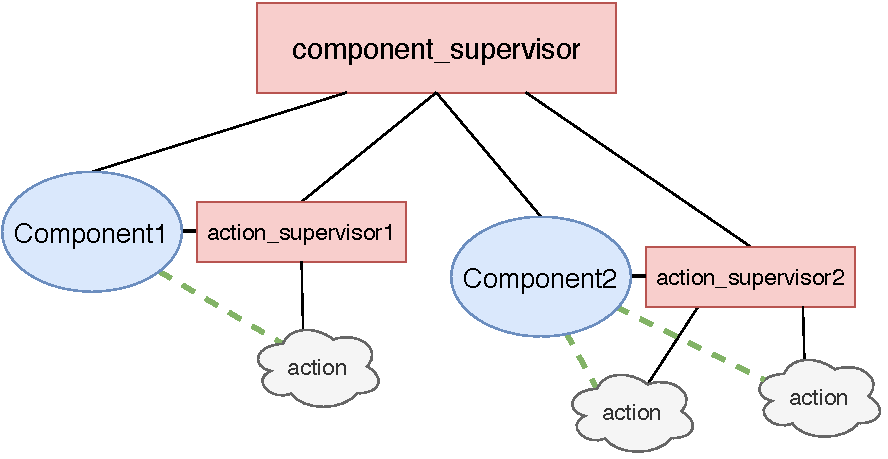
\includegraphics[width=0.7\linewidth]{implementation_details/component_and_action.pdf}
	\caption{Part of the overall supervision tree showing components with their actions and their relative Action Supervisor}
	\label{fig:component-and-action}
\end{figure}

Picture ~\ref{fig:component-and-action} shows a component with its actions in the supervision tree. Actions are attached to a specific supervisor (the Action Supervisor) which is unique for each component.
\\

\underline{The event Listener:}


A component module may have zero or more event listeners attached to the Event Manager. Event listeners are responsible for listening and forwarding internal events that are of interest to the component module.

A component that provides a service must have an event listener in order to receive requests from other components. Event listeners are event handlers in Erlang terminology.

\begin{figure}
	\centering
	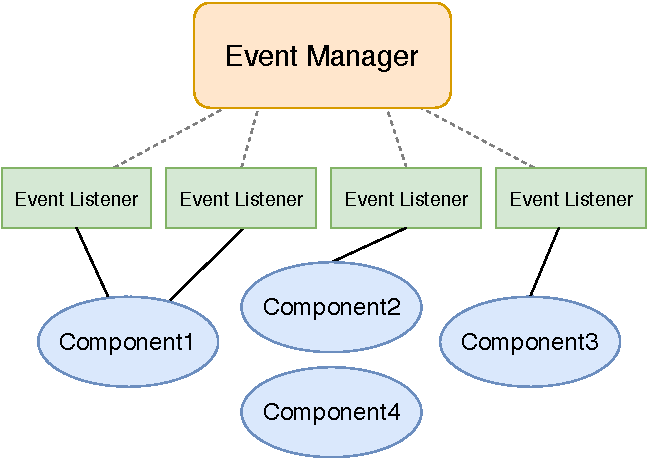
\includegraphics[width=0.7\linewidth]{implementation_details/components_event_listeners.pdf}
	\caption{Components with Event Listeners registered on the Event Manager}
	\label{fig:component-event-listeners}
\end{figure}


Figure ~\ref{fig:component-event-listeners} shows how event listeners are attached to components and registered on the Event Manager.
Note that Component4 doesn't have any event listener, which is a perfectly valid situation.

\subsubsection{Coordinator}

The Coordinator represents the logic and reasoning of the system, coordinating the various components in order to achieve the vehicle’s goals.

The Coordinator listens for internal events of interest by registering event listeners on the Event Manager (just like components do).
Specific internal events trigger the Coordinator's actions which, in turn, produce new internal events addressed to specific components. 

This behaviour of recognising specific events and addressing specific components is what drives the vehicle towards its goals.

\subsubsection{The general flow of events}

Once the vehicle has been initialized and the startup message received the vehicle can begin to move. 
\\

(1)The Coordinator starts by asking the Recognition Component about the position type it is currently on. 
\\

There can be 2 basic position types (although the implementation provides significantly more) a \textit{free} position and a \textit{stop} position.

A \textit{free} position is any position onto which the vehicle is free to advance (for example, it is on a public road), where as a \textit{stop} position is a position that requires the vehicle to stop and resolve the situation (for example, an intersection entrance, an obstacle on the road, a 
car accident in front, etc).
\\

The Recognition Component utilises, for example, a camera system to detect the position type and returns the answer to the Coordinator.
\\

If the answer is \textit{free}, the Coordinator requests the Motion Component to check the position in front whether the vehicle is safe to advance.
If the answer is \textit{stop} the vehicle has to stop and resolve the problem. For the sake of simplicity (and, for the scope of this project) we assume that a position has type \textit{stop} if the vehicle is at the entrance to an intersection.
\\

 (2)Suppose that the Recognition Component's answer was \textit{free}, the Coordinator requests the Motion Component to verify the position in front. The Motion Component uses a proximity sensor to check whether the position in front is clear or occupied. The answer is provided to the Coordinator.
\\

If the answer is \textit{clear}, the vehicle advances in the next position. If the answer is \textit{occupied} the vehicle has to realise what is in front. For the scope of this project, we assume that only vehicles can be on the road. Therefore the vehicle tries to communicate with the vehicle in front, in order to check its health. The Coordinator requests the Communication Component to contact the vehicle in front.
\\

The Communication Component can use, for example, a Bluetooth device or a Wifi device to communicate with the vehicle in front (for example, send a broadcast with a message: "Who is at position X?"). The vehicle in front can either respond to the call, or, if it has software crashed, not respond at all. An answer is provided to the Coordinator.
\\

The Coordinator can either receive that the vehicle in front is \textit{up} (software is running correctly and the vehicle is waiting in a queue) or  \textit{down} (the vehicle in front has software crashed). If the vehicle in front is \textit{up}, the vehicle awaits in queue for the vehicle in front to move. If the vehicle in front is \textit{down} the vehicle calls a tow truck to remove the vehicle in front and awaits its removal.
In either cases, after a period of waiting, the vehicle moves in the position in front and the algorithm starts from (1).
\\

Returning to the step when the Coordinator requests the position type. If the Recognition Component’s answer is \textit{stop}, the vehicle is at the entrance to an intersection (for the reasons stated above) and has to stop to resolve the intersection crossing with vehicles at the other entrances in order to avoid potential collisions.
\\

The Coordinator uses the Communication Component in order to solve the intersection. The Communication Component contacts the intersection participants (vehicles at the entrances) and starts the intersection coordination (described in the next section). Once the vehicle is clear to move in the intersection, a notification is made to the Coordinator that the current position is \textit{free} and the algorithm takes on from (2).

\subsection{Intersection Coordination}

\subsection{Vehicle Generator}


\chapter{Validation}
The validation part consisted in three main phases. First of all the project was tested with few vehicles generated singularly into different shells, with Erlang nodes created on local machine. After the initial validation, simulating peculiar situation manually (software and mechanical failures, vehicles arrival at specific times, \dots), the software has undergone numerous tests with the help of the vehicle generator described in the previous chapter, even this with Erlang nodes on local machine. Finally, exploiting Docker facilities, we tested the project even in distributed containers on different hosts in a virtual network.

The project has been tested on Fedora 30 with Erlang/OTP 21, and on Ubuntu 18.04 LTS with Erlang/OTP 22.

After careful planning and developing, and after all these tests phases, we are confident of providing a reliable and sound solution. In next sections is described how to reproduce the tests. All the scripts provided have been tested only on cited above operative systems, same results are not guaranteed in Mac OS or Windows.

To perform tests is necessary to have in mind the graph of the interception presented in Figure~\ref{fig:config-graph}. Moreover, for the test with the generator and with docker, the scripts will not exit at the end of the simulation, because we can't understand when all vehicles have finished, but you can easily check that if for about a minute nothing is printed, then the simulation is over, and you can kill the script with \verb|ctrl+C| and then \verb|(a)bort|.

\section{Simple Tests}
To use the code proposed here is necessary to execute \texttt{make all}. Some scripts are provided in the direcotry \texttt{test/}. Note that is is important to execute the script provided from the project root.

First of all it is necessary to start the environment. To do it open a shell and run:
\begin{verbatim}
./test/start_environment.sh
\end{verbatim}
You should se now an Erlang shell with the message ``Env started!''.

Now it is time to produce vehicles: pretty easy, open another shell and run:
\begin{verbatim}
./test/start_vehicle.sh 1 R_1 R_30
\end{verbatim}
Where, the first parameter is the index of the vehicle to generate --- note that if you insert $x$ the erlang node will be \verb|v|$x$\verb|@hostname|. The second and the third parameters are the start position, and the destination position, chosen from the graph in Figure~\ref{fig:config-graph}. One can also start a vehicle from other positions chosen from $R_x$ or $IN_x$, to test different situations.

You will see that in every vehicle shell is printed what it is doing, and more information can be found in the vehicle logs inside the \texttt{log/} directory.

\section{Vehicle Generator}
To use the code proposed here is necessary to execute \texttt{make all}. To start the vehicle generator can be used the script inside the \texttt{test/} directory, as follows:
\begin{verbatim}
./test/start_generator.sh <vehicle number> <fail ratio> \
	[relaive sw fail ratio] [max fail timeout (ms)]
\end{verbatim}
for example you can try:
\begin{verbatim}
./test/start_generator.sh 10 0.2 0.5 20000
\end{verbatim}
Where:
\begin{itemize}
	\item \verb|<vehicle number>| is mandatory and represent the number of vehicles that will be generated.
	\item \verb|<fail ratio>| is mandatory and represent the percentage (expressed with a number $0 \le x \le 1$) of failures that will be generated.
	\item \verb|[relaive sw fail ratio]| is optional and represent the ratio of software failures caused by the generator. (e.g. if set to $0.5$, half faults will be software, and the other half will be mechanical).
	\item \verb|[max fail timeout (ms)]| represent the maximum time in milliseconds within which the fault will be caused, considering the moment when the vehicle starts. (e.g. if set to $20000$, the vehicle can fail after a maximum of $20s$ from its start).
\end{itemize}
To stop the execution press \verb|ctrl+C| and then \verb|(a)bort|. The information here are printed all in the same shell, so it is less clear what is happening, but the logs for each vehicle can be found in the \verb|log/| directory.

\section{Docker}
To use the code proposed here is necessary to execute \texttt{make docker}. Note that with the tests proposed here is required to have docker installed and configured properly. Some containers, and a network, will be created. In \verb|docker/| directory are provided some script to easily run the tests and also to stop and clean the containers and network created.

The command to run is:
\begin{verbatim}
./docker/start_docker.sh <vehicle number> <fail ratio> \
[relaive sw fail ratio] [max fail timeout (ms)]
\end{verbatim}
for example you can try:
\begin{verbatim}
./docker/start_docker.sh 10 0.2 0.5 20000
\end{verbatim}
Where the parameters are the same of the vehicle generator described in the previous section.
Note that in docker you will se only messages printed from the generator. To see what happens to the vehicles you can look at the \verb|docker_log/| directory, where all vehicles log are generated. Further, can be necessary to provide root permission to delete \verb|docker_log/| directory, because the files are generated by root user inside the containers, so the proprietary user is still root.
After stopping the simulation, everything can be cleaned with:
\begin{verbatim}
./docker/clean_docker.sh
\end{verbatim}

\chapter{Conclusions}
The proposed solution focuses on a very simplified version of what a real solution could be. In particular the aim was to produce a core solution which satisfies the requirements but that also does not contain more than necessary assumptions, and in particular that does not rely on non realistic ideas that can lead future development to a blind spot.

\section{Partial implementation and future work}
Some advancement that can be pursued starting from our solution are provided here. Some of them are easier than other, but due to lack of time we did not managed to deepen them:
\begin{itemize}
	\item Try different interception graphs;
	\item Centralize some configuration parameters in such a way the solution can be tuned without recompiling;
	\item Exploit code change feature offered by Erlang;
	\item Develop a graphical interface of the environment to better understand how vehicles are moving;
	\item Add vehicles with priorities, e.g. emergency vehicles;
	\item Dynamically modify paths inside the crossroad if some position becomes unavailable;
	\item Let more than one vehicle per time cross the intersection, maybe with an interface to a planner in order to find the best route (exploiting epistemic planning could be an interesting option).
\end{itemize}

\end{document}